\section{Methodology}
\label{sec:methodology}

% Avsnitt om hva slags type review dette er og hvorfor vi har valgt den typen
To ensure reproducible and unbiased results, this review follows a structured methodology. As noted by \textcite{tranfield_et_al}, traditional literature reviews often lack systematic rigor, making it challenging to determine the validity of their conclusions. To address this issue, each stage of the review was conducted systematically, guided by established literature review frameworks, particularly \textcite{snyder_2019} and \textcite{marzi_et_al_2024}. The review adopts a structured systematic literature review (SLR) approach in line with \textcite{snyder_2019}, ensuring that the review is exhaustive and able to identify the most important research gaps. 

The review design and screening process followed the proposed steps by \textcite{marzi_et_al_2024}: (1) defining research questions and boundaries, (2) defining search queries, (3) selecting databases, (4) screening and cross-checking data and (5) cleaning and exporting data. This approach aligns with the design and conduct phases proposed by \textcite{snyder_2019}. Holistic and specific cluster thematic analysis was subsequently conducted as per \textcite{marzi_et_al_2024}, while bibliometric analysis following their (B-SLR) framework was also conducted, but excluded due to uninformative results. The cluster topic identification method for the specific cluster thematic analysis suggested by \cite{marzi_et_al_2024} was considered but not pursued as the field is too small and fragmented for meaningful clusters to appear. Instead, a framework for breaking down the sample by the dimensions deemed important to answer the research questions was adopted. 

The exact process is outlined below, and reported according to \textcite{marzi_et_al_2024}'s guidelines.

% Avsnitt om databasevalg
\textbf{Database Selection}\nopagebreak

When doing a systematic review, it is important to conduct the search in a sufficient number of databases to ensure that all relevant articles are retrieved \parencite{hiebl_2021}. Furthermore, it is critical that the databases are relevant for the researched topic \parencite{marzi_et_al_2024}. In order to comprehensively capture all potentially relevant literature, this review utilized multiple well-establish databases: SCOPUS, Web of Science, IEEE Xplore and ProQuest. SCOPUS and Web of Science were chosen due to their extensive coverage and comprehensive indexing of academic literature within a wide range of fields, as well as being the most extensively used databases for reviews \parencite{marzi_et_al_2024}. IEEE Xplore was included being a leading database for review articles in the fields of computer science and engineering \parencite{suhaimi2020systematic, carvalho2019systematic, cavacini2015best}, while ProQuest is another large academic database utilized in line with \textcite{gunnarsson2024}. All chosen databases allowed for advanced search queries without limitations on the number of clauses, in contrast to for example Google Scholar and ScienceDirect. 

% Avsnitt om søkekriterier
\textbf{Search Strategy and Filtering Criteria}\nopagebreak

A comprehensive search and filtering strategy was developed to ensure the review covered all relevant literature. The search criteria were designed to ensure that as many articles relevant to the research questions as possible were included, as a narrow search query in this phase can lead to involuntary exclusion of relevant documents \parencite{marzi_et_al_2024,kuhrmann2017pragmatic, williams2021reexamining}. By requiring articles to match at least one term in four different clauses, the intention was to ensure that every article was (1) within the field of AI, (2) about probabilistic modeling, (3) about forecasting, and (4) within finance. Table \ref{table:keywords_used} shows all key words included within each clause. Conference papers, book chapters, editorials, and early access/unfinished papers were excluded to focus on peer-reviewed journal articles, which represent validated knowledge that has undergone peer review to ensure reliability \parencite{marzi_et_al_2024, hota2022hybrid}. Only English articles are included. The exact search queries are shown in Appendix \ref{appendix:search_queries}. 

\begin{table}[H]
    \centering
    \caption[Keywords used in database search queries]{Keywords used in database search queries across four key areas. Papers must match at least one term in each of the four categories to be included in the initial sample.}
    \label{table:keywords_used}
    \begin{adjustbox}{width=0.5\textwidth,center}
    \begin{tabular}{p{0.15\textwidth}p{0.35\textwidth}}
        \toprule
        \textbf{Category} & \textbf{Keywords\tablefootnote{The asterisk (*) is a wildcard character used for truncation of common endings to the same word }} \\
        \midrule
        (1) Artificial Intelligence (AI) & \texttt{AI, ML, Artificial intelligence, Machine learning, Deep learning, Reinforcement learning, Supervised learning} \\
        \addlinespace
        (2) Probabilistic Modeling & \texttt{Probabilistic, Uncertainty quantification, Prediction interval*, Confidence interval*, Distributional forecast, Bayesian, Gaussian process, Undirected graphical model*, Markov Network*, Markov random field*, Probabilistic Graphical Model*, Variational inference, Monte Carlo inference, Hidden Markov model*, Gaussian mixture model*, Variational Autoencoder*, Dirichlet Process} \\
        \addlinespace
        \text{(3) Forecasting} & \texttt{Forecast*, Predict*, Estimat*} \\
        \addlinespace
        \text{(4) Finance} & \texttt{Cryptocurrency, Bitcoin, Foreign exchange, Forex, Equity market*, Stock price*, Stock market*, Commodities, Value-at-risk, Value at risk, CVaR, Expected shortfall, Financial time series, Stock trend*, Implied volatility, Realized volatility, (Volatility AND financ*)} \\
        \bottomrule
    \end{tabular}
    \end{adjustbox}
\end{table}

The search was conducted across all the databases in October 2024, yielding a combined initial search result of 555 articles from all databases. The search results were then merged, and duplicates were removed, resulting in 326 unique articles. 

\begin{figure}[H]
    \centering
    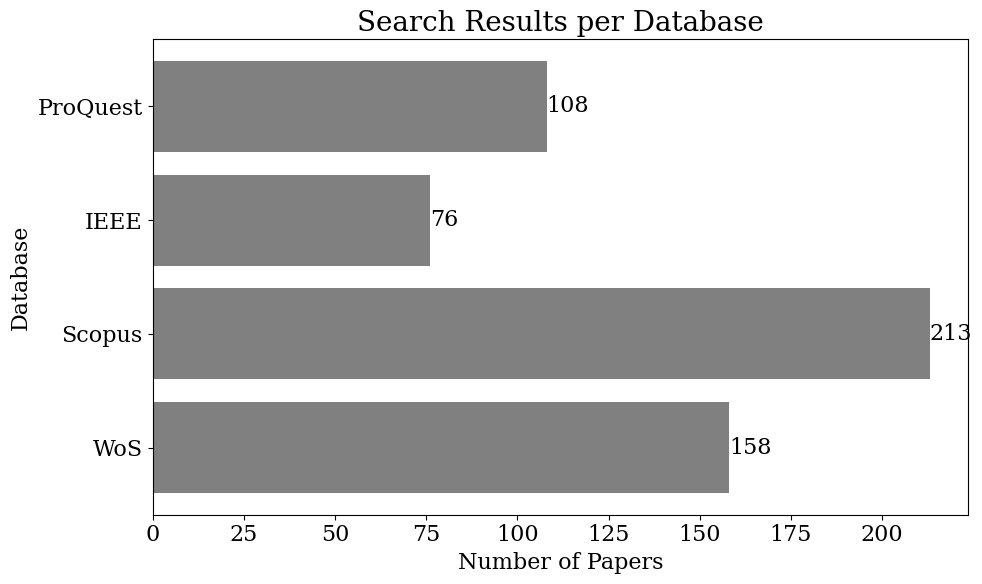
\includegraphics[width=1\linewidth]{Images/search_sample_by_database.png}
    \caption{Number of paper results per database based on search queries.}
    \label{fig:search_sample_by_database}
\end{figure}



% Avsnitt om screening
\textbf{Inclusion criteria}\nopagebreak

Following the definition of the search strategy, inclusion criteria for the screening process was defined. Three main criteria were defined for the first screening phase:

\begin{enumerate}
    \item The article must discuss a model that predicts the price of some financial instrument (e.g. a stock, an option, an index, etc.)
    \item The model must be an AI or machine learning model, i.e. more complicated than traditional statistical or econometric models
    \item The model must be able to provide more than a point prediction, i.e. it includes either variance, a distribution or some other financial risk measure such as VaR
\end{enumerate}

Furthermore, some explicit rules in cases of doubt in the aforementioned three was constructed:
\begin{itemize}
    \item Articles focusing on commodities were included only if they predicted futures prices, except for gold and oil, which closely resemble financial time series and correlate with financial variables \parencite{Gokmenoglu2015}
    \item Studies must demonstrate practical implementation of the proposed models, not merely discuss theoretical frameworks
    \item To distinguish between traditional statistical models and AI/ML models, we classified models as AI/ML if they demonstrated complexity beyond Bayesian Structural Time-Series (BSTS) and required machine learning estimation techniques, such as gradient descent
    \item Unlike \textcite{Blasco_et_al_2024}, we excluded models that use probabilistic components solely for purposes such as regularization (e.g., most Bayesian Regularized Neural Networks and Neural Networks with dropout during training), optimization, or feature extraction. As \textcite{Blasco_et_al_2024} observed, these articles rarely quantify uncertainty. This exclusion is the primary reason our sample size is smaller than that of \textcite{Blasco_et_al_2024}, despite our broader scope and longer time range
    \item Classification models were only included if they used methods explicitly designed for probability estimation or made efforts to improve probability calibration. Models inherently providing well-calibrated probabilities, such as Bayesian Networks and HMMs were included
    \item MLPs/FFNNs with Gaussian activation functions were excluded, as they do not provide probabilistic estimates
\end{itemize}
These became especially relevant during screening phase 2 when full-text screening was conducted. 

\textbf{Screening Phase 1: Initial Screening}\nopagebreak

After obtaining the initial set of papers, the Phase 1 screening process started. In this stage, the purpose was to remove articles irrelevant to the research questions to be addressed in the review.

To make the screening process more efficient, a large language model (``o1-mini'' from OpenAI) was given the title and abstract of each article and tasked with generating a short summary and assessing compliance with each criteria. Subsequently, the results from the language model, along with the title, abstract and a link to the full article was given to one of the researchers to make a decision on whether to include or exclude each article. Through this process, we were able to quickly make decisions on obvious cases, and do a more thorough assessment where we potentially could open and skim through the article in cases of doubt, thus enabling us to screen a large number of articles in a short amount of time, and making thorough assessments that were not based solely on the title and the abstract. The exact process is outlined in Appendix \ref{appendix:screening_process_with_ai} and the code used is published at \href{https://github.com/tjespe/literature-review/}{Github}\footnote{\label{footnote:github_link}\href{https://github.com/tjespe/literature-review/}{https://github.com/tjespe/literature-review/}}. Through this process, the number of articles in the sample was reduced from 326 to 133.

% Avsnitt om snowball effect - XX articles were added to sample by snowball effect



% Avsnitt om den initielle analysen (taggingen)
\textbf{Screening Phase 2: Full-text screening, Data extraction and Analysis}\nopagebreak

Following the initial screening and dataset extraction, a second, more comprehensive screening was conducted, involving full-text review and thorough evaluation of each article. Data was extracted on key information about each article, such as the type of probabilistic model used, any hybrid model integrations, target variable, type of uncertainty addressed, metrics used for assessing uncertainty estimates, how the model compared to benchmarks etc. Each article was tagged and categorized based on these variables which were summarized in a structured format for subsequent analysis and descriptive statistics. 

In this detailed evaluation a deeper understanding of each article and its model implementation was achieved, leading to the exclusion of several articles not passing the aforementioned criteria after all. These exclusions were not identifiable during the initial screening, mostly due to the difficulty of fully understanding the model implementation details before reading full-text. Typical exclusions in this phase was: the model could not be considered AI or ML after all, the model architecture was only discussed and not actually implemented, the model did not actually have the ability to produce probabilistic outputs, or the model predicted categories without well calibrated probabilities. Therefore, the final sample size of included articles presented in this paper is \samplesize articles. Figure \ref{fig:screening_and_cleaning_funnel} illustrates how the sample size was reduced down through the cleaning and screening. 

  \begin{figure*}[h]
      \centering
      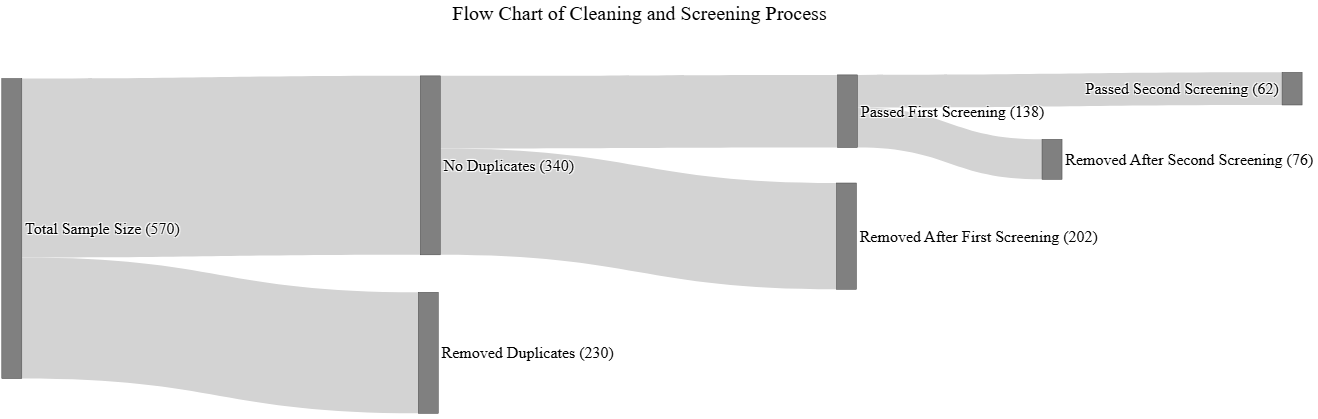
\includegraphics[width=1\linewidth]{Images/screening_funnel.png}
      \caption{Flow chart illustrating the sample size throughout cleaning and screening phases.}
      \label{fig:screening_and_cleaning_funnel}
  \end{figure*}


  % Avsnitt om hvordan deskriptiv statistikk ble laget og hvorfor, inkl. analysen som viste at de sjeldent referer til hverandre, med referanse til den B-SLR-artikkelen
\textbf{Descriptive Statistics and Analysis}\nopagebreak

Descriptive statistics and analysis were generated using a Python Jupyter Notebook for the final sample of papers. Pandas was used for data manipulation and categorization, and Matplotlib for data visualizations and plotting. All code used for the analyses is disclosed and available for reproducibility at \hyperlink{https://github.com/tjespe/literature-review/}{Github}\textsuperscript{\ref{footnote:github_link}}.

% Avsnitt om den videre analysen (altså breakdown by model, by target variable, etc.): hvorfor og hvordan har vi gjort det?
\textbf{Approach for Further Analysis}\nopagebreak

The further analysis of the papers follows a structured breakdown along several dimensions: type of model, output of model, asset class and type of uncertainty. Each section will provide insights that inform the research questions before concrete conclusions are presented for each question in Section \ref{sec:discussion}. The dimensions used to analyze the sample align with those commonly employed in similar reviews, providing a structured framework to effectively assess the current state of research \parencite{Blasco_et_al_2024}.

